\documentclass{beamer}
%\documentclass{powerdot}
%\documentclass{slides}[14pt]
%\pagestyle{empty}
%\normalsize
\usepackage{amsmath}
\usepackage{amssymb}
\usepackage{amscd}
% \usepackage{moreverb}
\usepackage{graphicx}
% \usepackage[all]{xy}
% \usepackage{beamerthemesplit}
\usepackage{moreverb}
\usepackage[all]{xy}

\input macros			   %% loan from John Gibson's snowbird 07 talk
% \input ../../inputs/defsThesis     %% all Vaggelis edits: \renewcommand, etc

% Setup appearance:

\usetheme{Darmstadt}
\usefonttheme[onlylarge]{structurebold}
\setbeamerfont*{frametitle}{size=\normalsize,series=\bfseries}
\setbeamertemplate{navigation symbols}{}


% Standard packages

\usepackage[english]{babel}
\usepackage[latin1]{inputenc}
\usepackage{times}
\usepackage[T1]{fontenc}


% % Setup TikZ
%
% \usepackage{tikz}
% \usetikzlibrary{arrows}
% \tikzstyle{block}=[draw opacity=0.7,line width=1.4cm]

\title{Continuous symmetry reduction for high-dimensional flows}
\author{Evangelos Siminos}
\author[Siminos, Cvitanovi\'c, Davidchack]
{
  \textcolor{green!50!black}{
  {Predrag~Cvitanovi\'c}\inst{1}
  and
  {Evangelos~Siminos}\inst{1,2}
  }
}
\institute
{
  \inst{1}%
  Georgia Institute of Technology
  \and
  \vskip-2mm
  \inst{2}
  CEA/DAM/DIF, Paris
}
\date{April 2, 2010}

\begin{document}

\begin{frame}
  \titlepage
\end{frame}

\begin{frame}{Outline}
  \tableofcontents
\end{frame}


\section[KSe]{\KSe}

\subsection{\KSe\ as a baby Navier-Stokes}
\begin{frame}{\KSe}

\begin{block}{1-dimensional ``Navier-Stokes''}
\[
  u_t + u \triangledown u \,=\, -\triangledown^2 u- \triangledown^4 u
    \,,\qquad   x \in [-L/2,L/2]
    \,,
\]
\end{block}

describes extended systems such as
\begin{itemize}
 \item reaction-diffusion systems
 \item combustion problems (flame fronts)
 \item drift waves in plasmas
 \item thin falling films
 \item and more\ldots
\end{itemize}

\end{frame}

\begin{frame}{Large $L$ \KSe\ solution}

\begin{center}
  \includegraphics[width=0.9\textwidth,height=0.5\textheight,clip=true]{../../figs/ks_largeL_cbar.eps}
\end{center}

\begin{itemize}
\item turbulent behavior
\item simpler physical, mathematical and computational setting than Navier-Stokes
\end{itemize}

\end{frame}


\section[Dynamicist's view of turbulence]
{Dynamical systems approach to spatially extended systems}

\begin{frame}{}
 \begin{itemize}
  \item understanding of chaotic dynamics: Rely on compact invariant objects.
  \item low dimensional systems: Equilibria and periodic
  orbits organize the long time dynamics.
  \item is this true in extended systems?
 \end{itemize}

\end{frame}


\subsection{Lorenz equations example}

\begin{frame}{From Lorenz attractor to a unimodal map}
	\begin{columns}[t]
	\column{.4\textwidth}
		\only<1>{
			\begin{exampleblock}{Lorenz equations}
					\[
% 	 			\dot{\ssp}=\vel(\ssp)
% 				=
				\left[
					\begin{array}{c}
				\dot{x} \\ \dot{y} \\ \dot{z}
				\end{array}
				\right]
				=
				\left[
					\begin{array}{c}
				\sigma (y-x) \\
				\rLor x - y -xz \\
				xy -bz
				\end{array}
				\right]
				\]
			with $\sigma = 10, b= 8/3, \rLor = 28$.
			\end{exampleblock}
		}
		\only<2>{
			 \begin{block}{Equilibria}
			 \[
		          \dot{\ssp}=\vel(\ssp)=0
		         \]
			\end{block}
		}
		\only<2,3>{
			\begin{block}{Linear stability of equilibria}
			 \[
			  A_{ij}=\frac{\partial \vel_i}{\partial \ssp_j}(x_{E_m})
			 \]
			\only<3>{
				Eigenvalues of A: $\eigExp[j]= \eigRe[j] \pm i\eigIm[j]$
				\begin{itemize}
				\item Linearly stable if $\eigRe[j]<0$
				\item Linearly unstable if $\eigRe[j]>0$
				\end{itemize}
			}
			\end{block}
			}
		\only<4>{
			\begin{block}{}
			$E_{0}:~
				\begin{array}{lcr}
					\eigExp[1] &=&11.83\\
					\eigExp[2] &=&-2.66\\
					\eigExp[3] &=&-22.83
				\end{array}
			$
			 \hspace{-0.2\textwidth}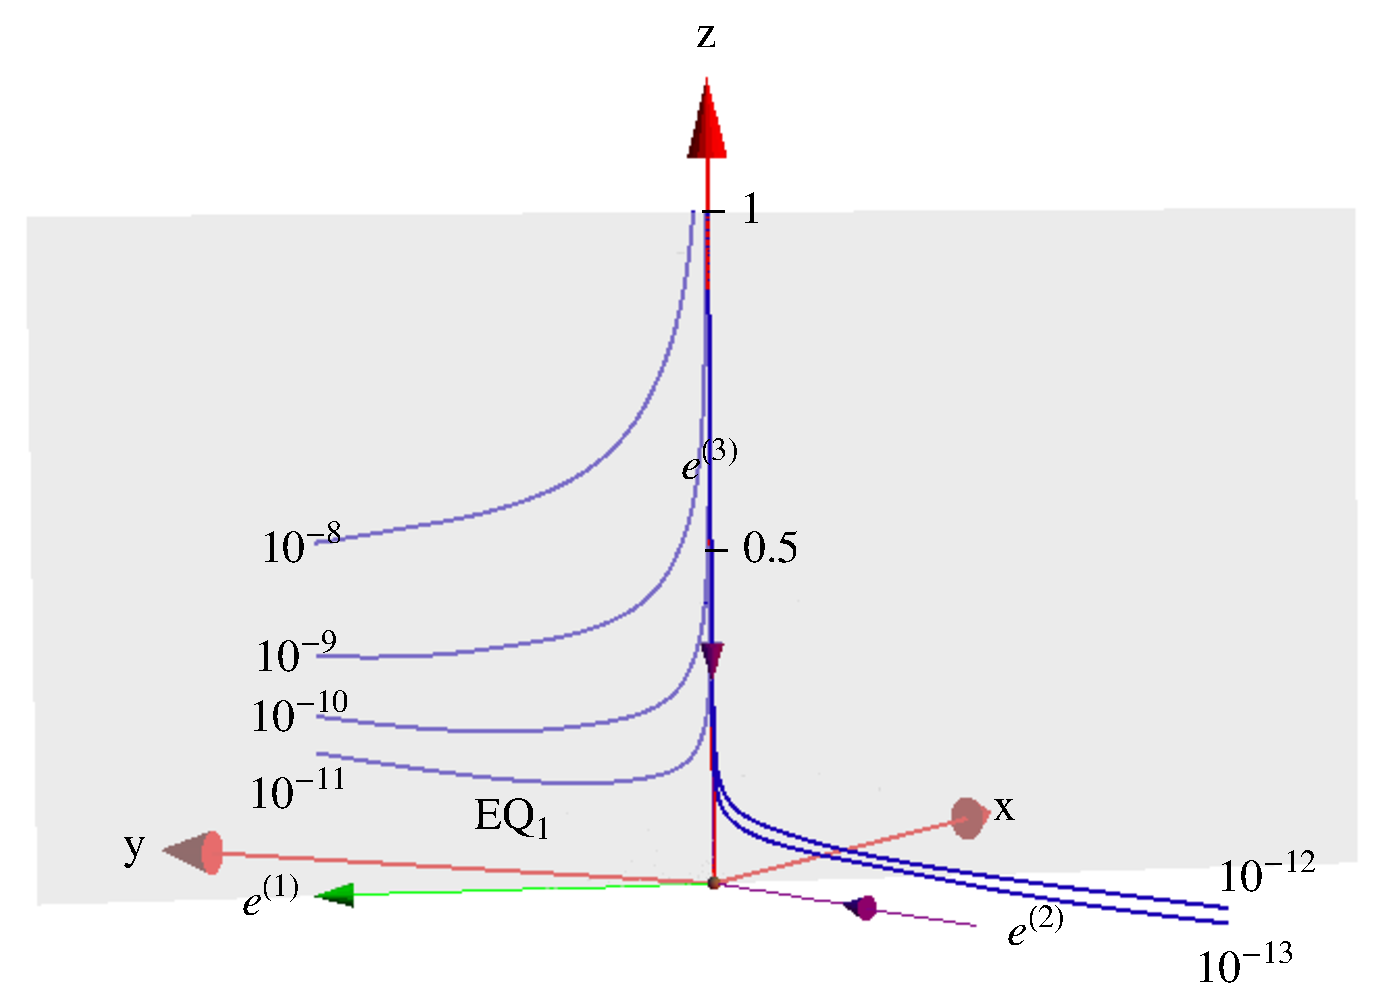
\includegraphics[width=1.2\textwidth,clip=true]{../../figs/lorenzSaddle0}
			\end{block}
		}
		\only<5>{
			\begin{block}{$E_{1}$}
			$\begin{array}{rcl}
					\eigExp[1,2]&=&0.094\pm10.19\\
					\eigExp[3] &=&-13.85
			\end{array}
			$
			 \hspace{-0.2\textwidth}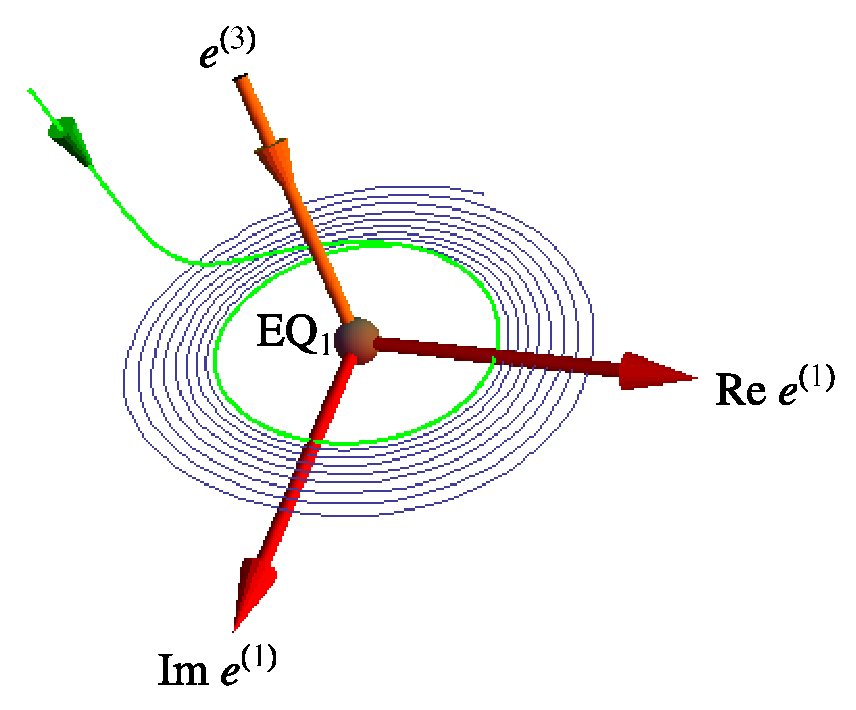
\includegraphics[width=1.2\textwidth,clip=true]{../../figs/lorenzPolarManifDetail1}
			\end{block}
		}
		\only<6>{
			\begin{block}{Poincar\'e section}
				$\mathcal{P}:$ (N-1)-dimensional hypersurface.
			\end{block}
			\begin{block}{Poincar\'e map}
			 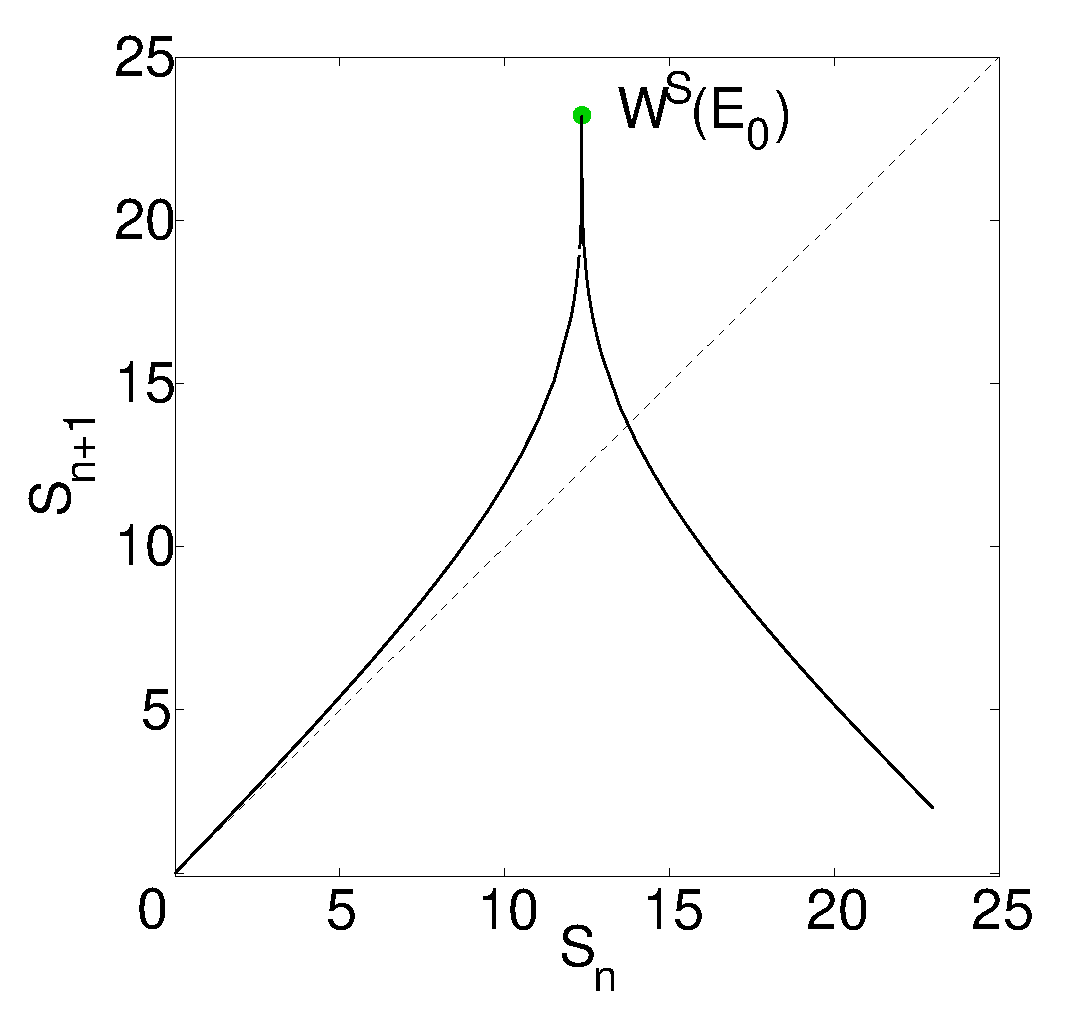
\includegraphics[width=\textwidth,clip=true]{../../figs/plorenz_retmap2}	
			\end{block}
			}
	\column{.55\textwidth}
		\begin{exampleblock}{Lorenz attractor}
			\only<1-5>{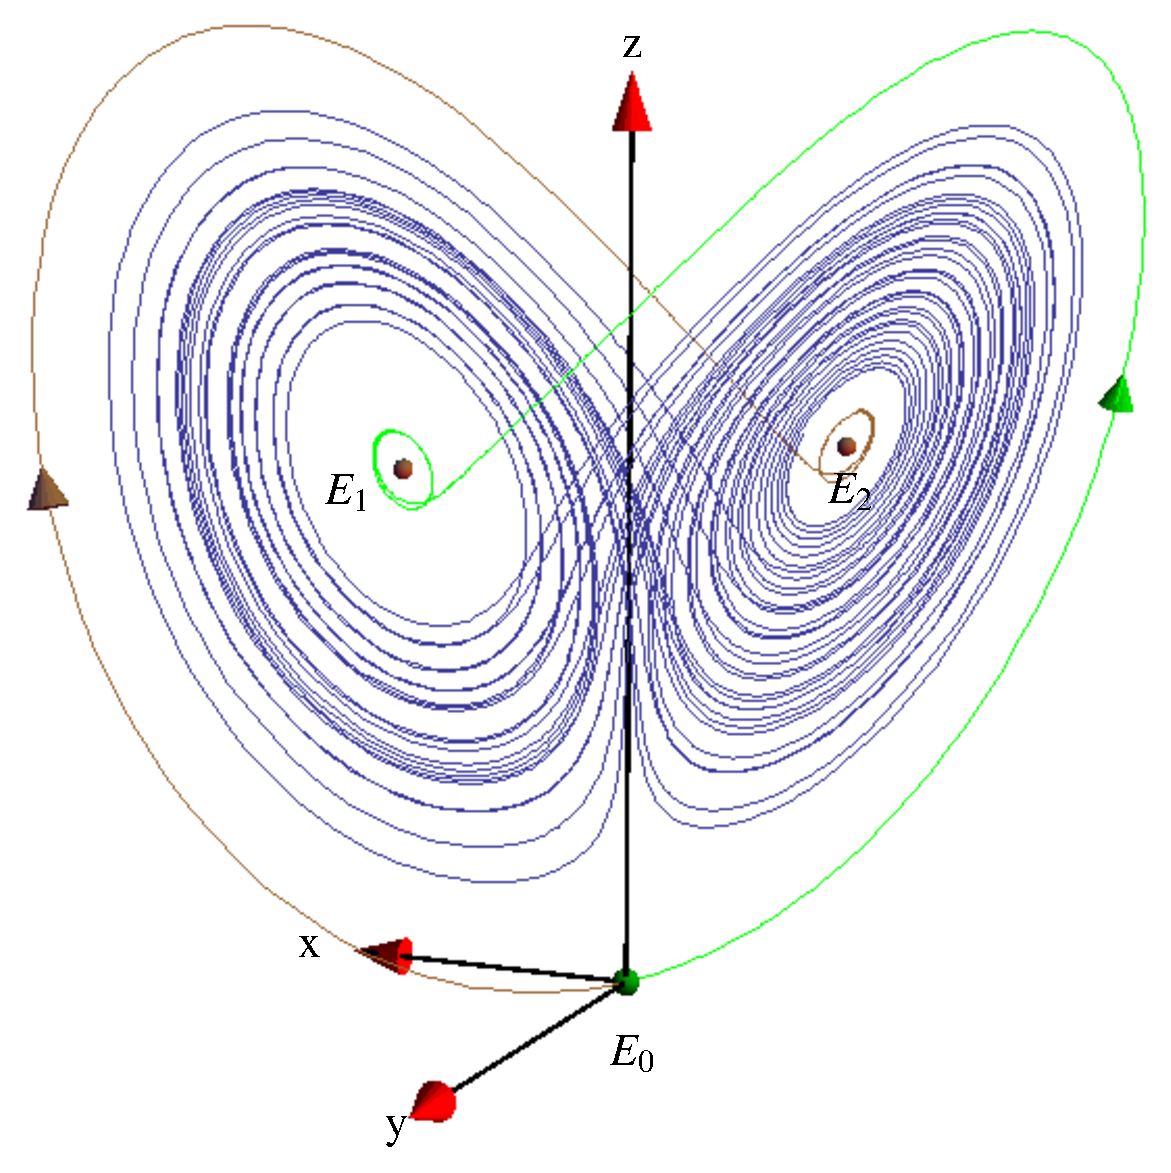
\includegraphics[width=\textwidth,clip=true]{../../figs/lorenzAttr}}
			\only<6>{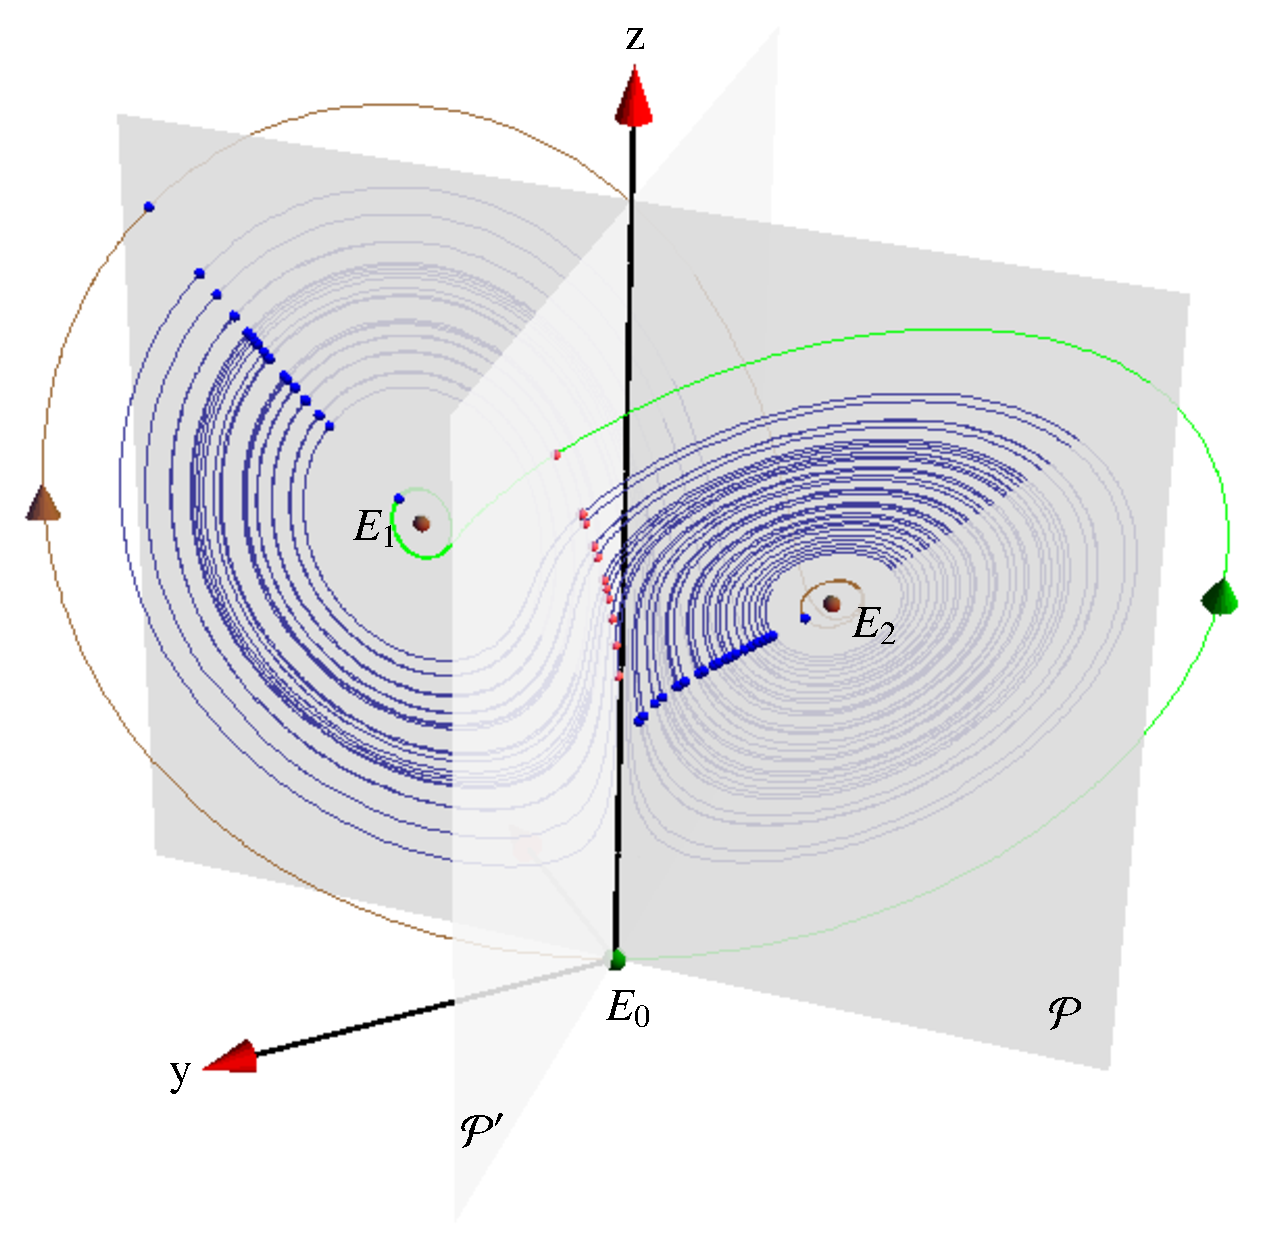
\includegraphics[width=\textwidth,clip=true]{../../figs/lorenz2Poinc}}
		\end{exampleblock}
	\end{columns}
\end{frame}


\subsection{PDE's as dynamical systems}

\begin{frame}

\begin{block}{State space}
 \begin{itemize}
	\item the space in which all possible states $\ssp$ live
	\item $\infty$-dimensional: A point $\phi(x)$ is a function of $x$ to be specified
		over an interval in $x$.
	\item In practice: a high but finite dimensional space
     (e.g. through a spectral discretization)
 \end{itemize}
\end{block}

\begin{block}{Intrinsic dimensionality}
 \begin{itemize}
  \item dynamics are often captured by fewer variables than
        needed to numerically resolve the PDE.
  \item how do we exploit such low dimensionality to obtain
  dynamical systems description?
 \end{itemize}
\end{block}

\end{frame}


\begin{frame}{{\KSe} reduced to discrete maps}
  \begin{block}{Take the hint from low dimensional systems}
  \begin{columns}
  \column{0.5\textwidth}
	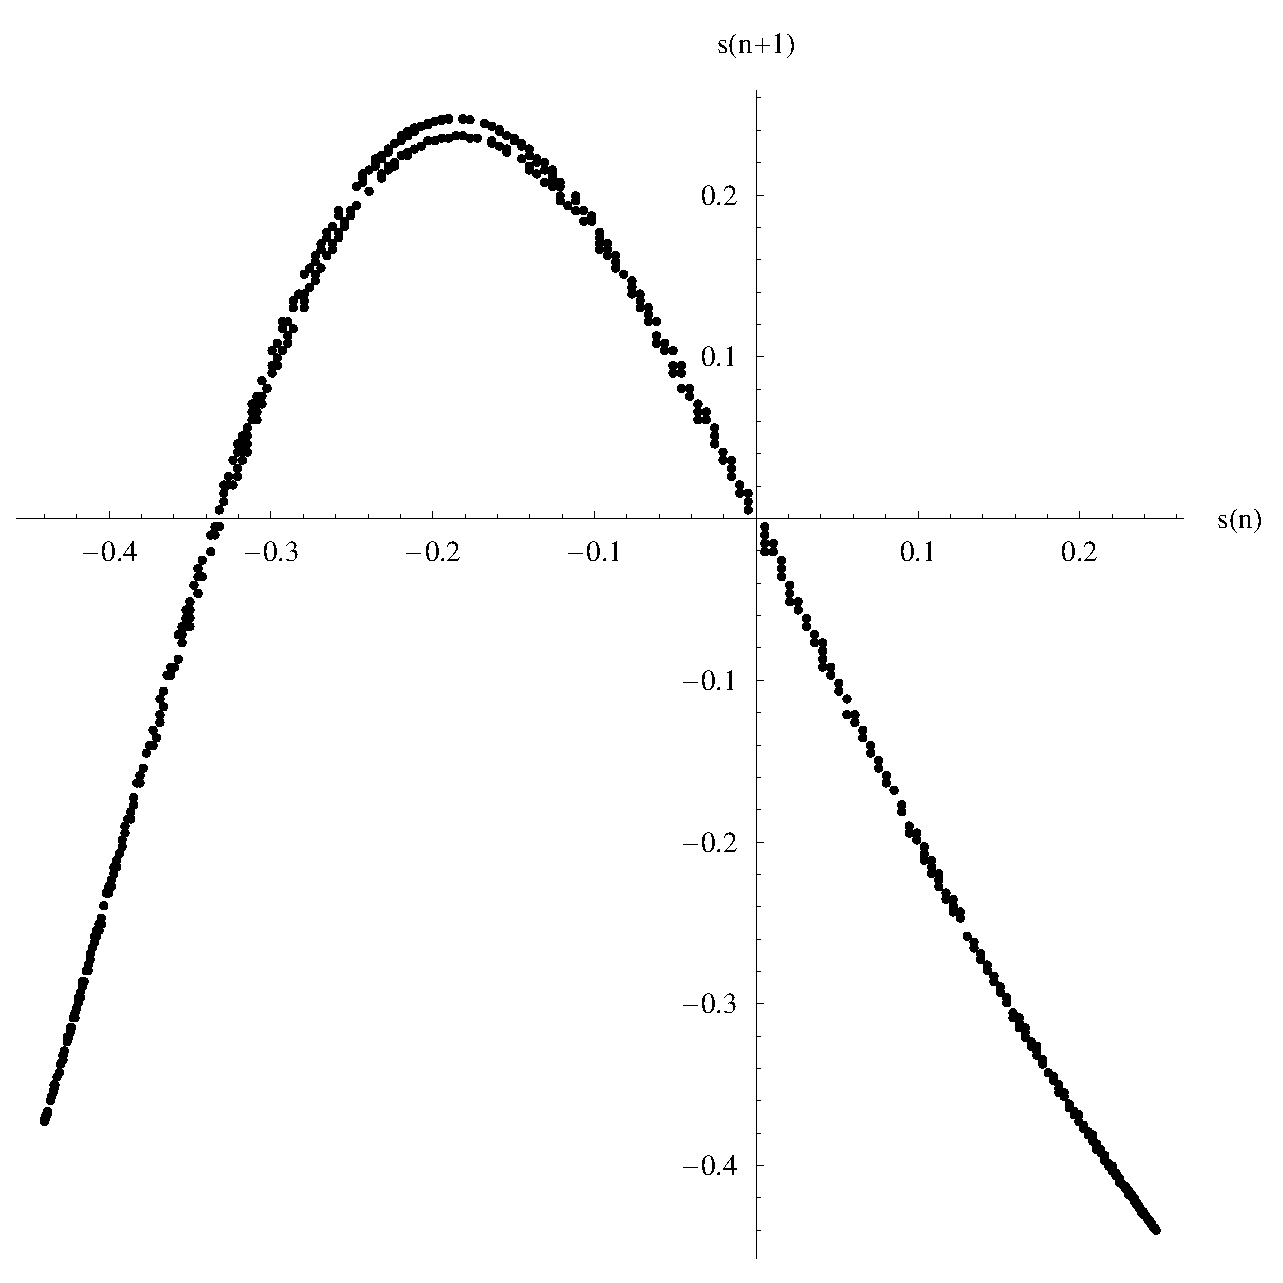
\includegraphics[width=\textwidth,clip=true]{../../figs/sPoincarePlot.eps}\\
	Christiansen et. al. (1996)
  \column{0.5\textwidth}
	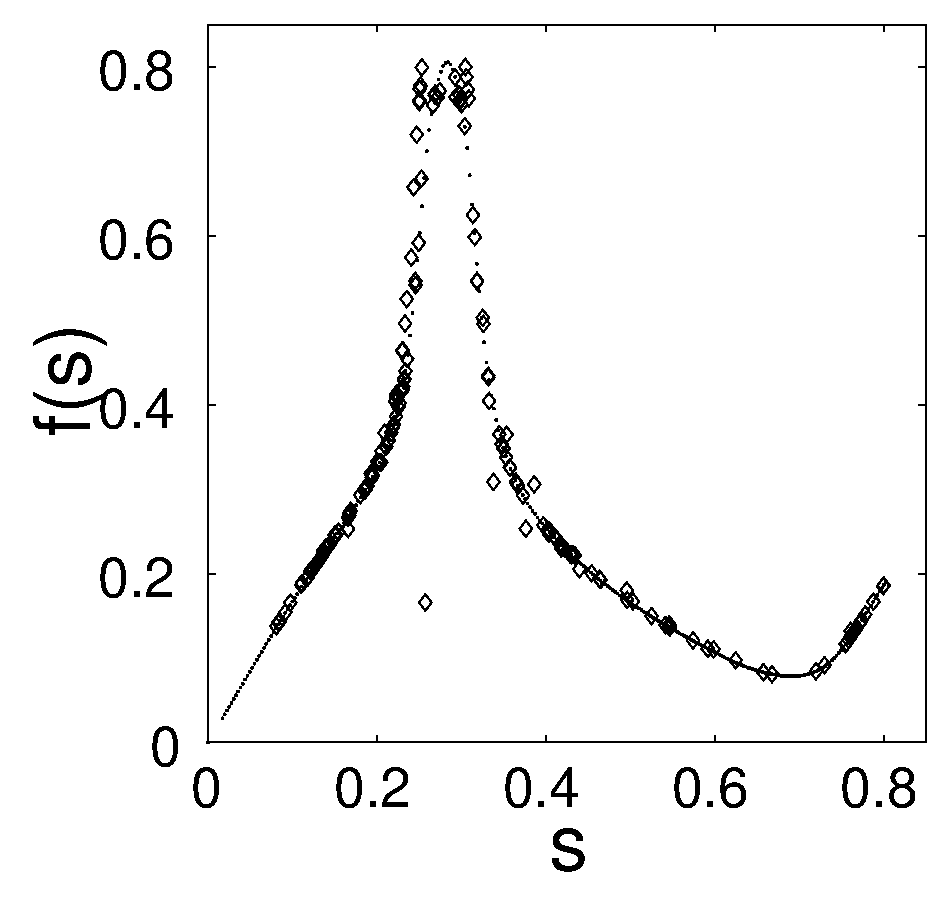
\includegraphics[width=\textwidth,clip=true]{../../figs/lanRM}\\
	Lan and Cvitanovi\'c (2004)
 \end{columns}
 \end{block}
\end{frame}




\begin{frame}{Symmetries of \KSe}

Impose periodic boundary conditions:
\[
 u(x,t) = u(x+L,t)
\]

Symmetry group $\On{2}$:
\begin{itemize}
 \item Translations: $\Shift_{\shift/L}\, u(x,t) = u(x+\shift,t)\,,\qquad \shift\in\left[-L/2,L/2\right]\,,$
 \item Reflections:  $\Refl \, u(x) = -u(-x)\,.$
\end{itemize}

Due to translational symmetry: traveling wave solutions.

\begin{block}{Question}
What are the invariant objects that organize phase space in a spatially extended system
with translational symmetry and \textcolor{green}{how do they fit together to form a
skeleton of the dynamics?}
\end{block}

\end{frame}



\section[KSe, $L=22$]{\KS, $L=22$, state space }

\subsection{$L=22$ solutions}

\begin{frame}{L=22}
\begin{center}
  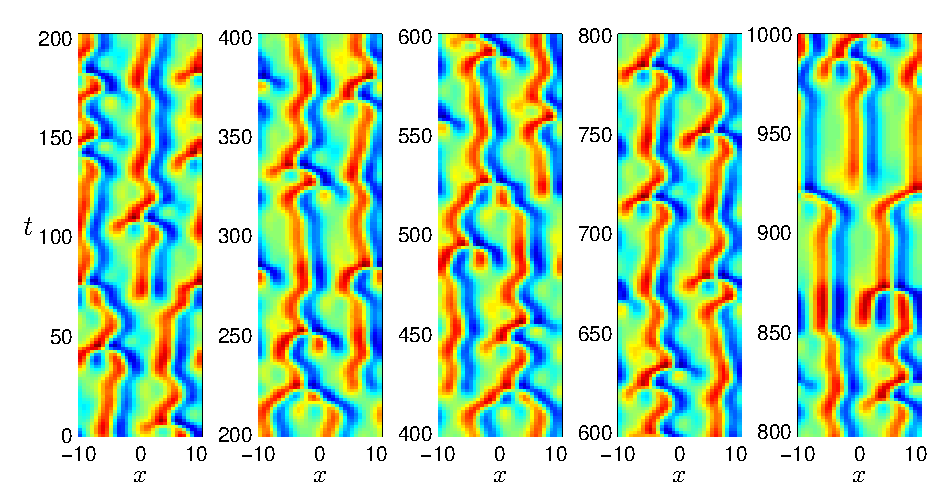
\includegraphics[width=0.9\textwidth,clip=true]{../../figs/ks_L22_long_orbit}
\end{center}

\begin{block}{}
 \begin{itemize}
  \item Lyapunov exponents: \\
	$(\lambda_i) = (0.048,$ 0, 0, $-0.003$, $-0.189$, $-0.256$, $-0.290$, $-0.310$, $\cdots)$
  \item Non trivial but tractable.	
 \end{itemize}

\end{block}

\end{frame}


\begin{frame}{Equilibria}
\begin{tabular}{ccc} ~~~\EQV{1} & ~~~\EQV{2} & ~~~\EQV{3} \vspace{12pt}\\
    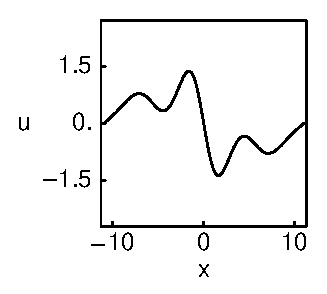
\includegraphics[width=0.25\textwidth,clip=true]{../../figs/1wKS22equil}&
    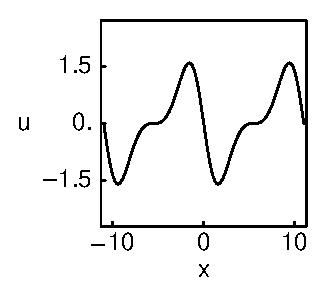
\includegraphics[width=0.25\textwidth,clip=true]{../../figs/2wKS22equil}&
   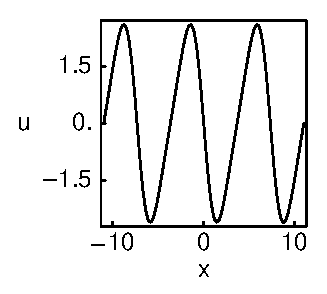
\includegraphics[width=0.25\textwidth,clip=true]{../../figs/3wKS22equil}
\end{tabular}

\begin{itemize}
 \item $\EQV{0}:\,u(x,t)=0$.
 \item $\EQV{3}$ invariant under $\Shift_{1/3}$.
 \item For any $\EQV{i}$ we have a continuous family of
 equilibria under rotations $\Shift_{\shift/L}\,\EQV{i}$.
 that live in $\Shift_{\shift/L}\,\bbU$.
\end{itemize}

\end{frame}



\begin{frame}{Traveling waves}
 \begin{columns}
 \column{0.4\textwidth}
%  \begin{tabular}{cc}
 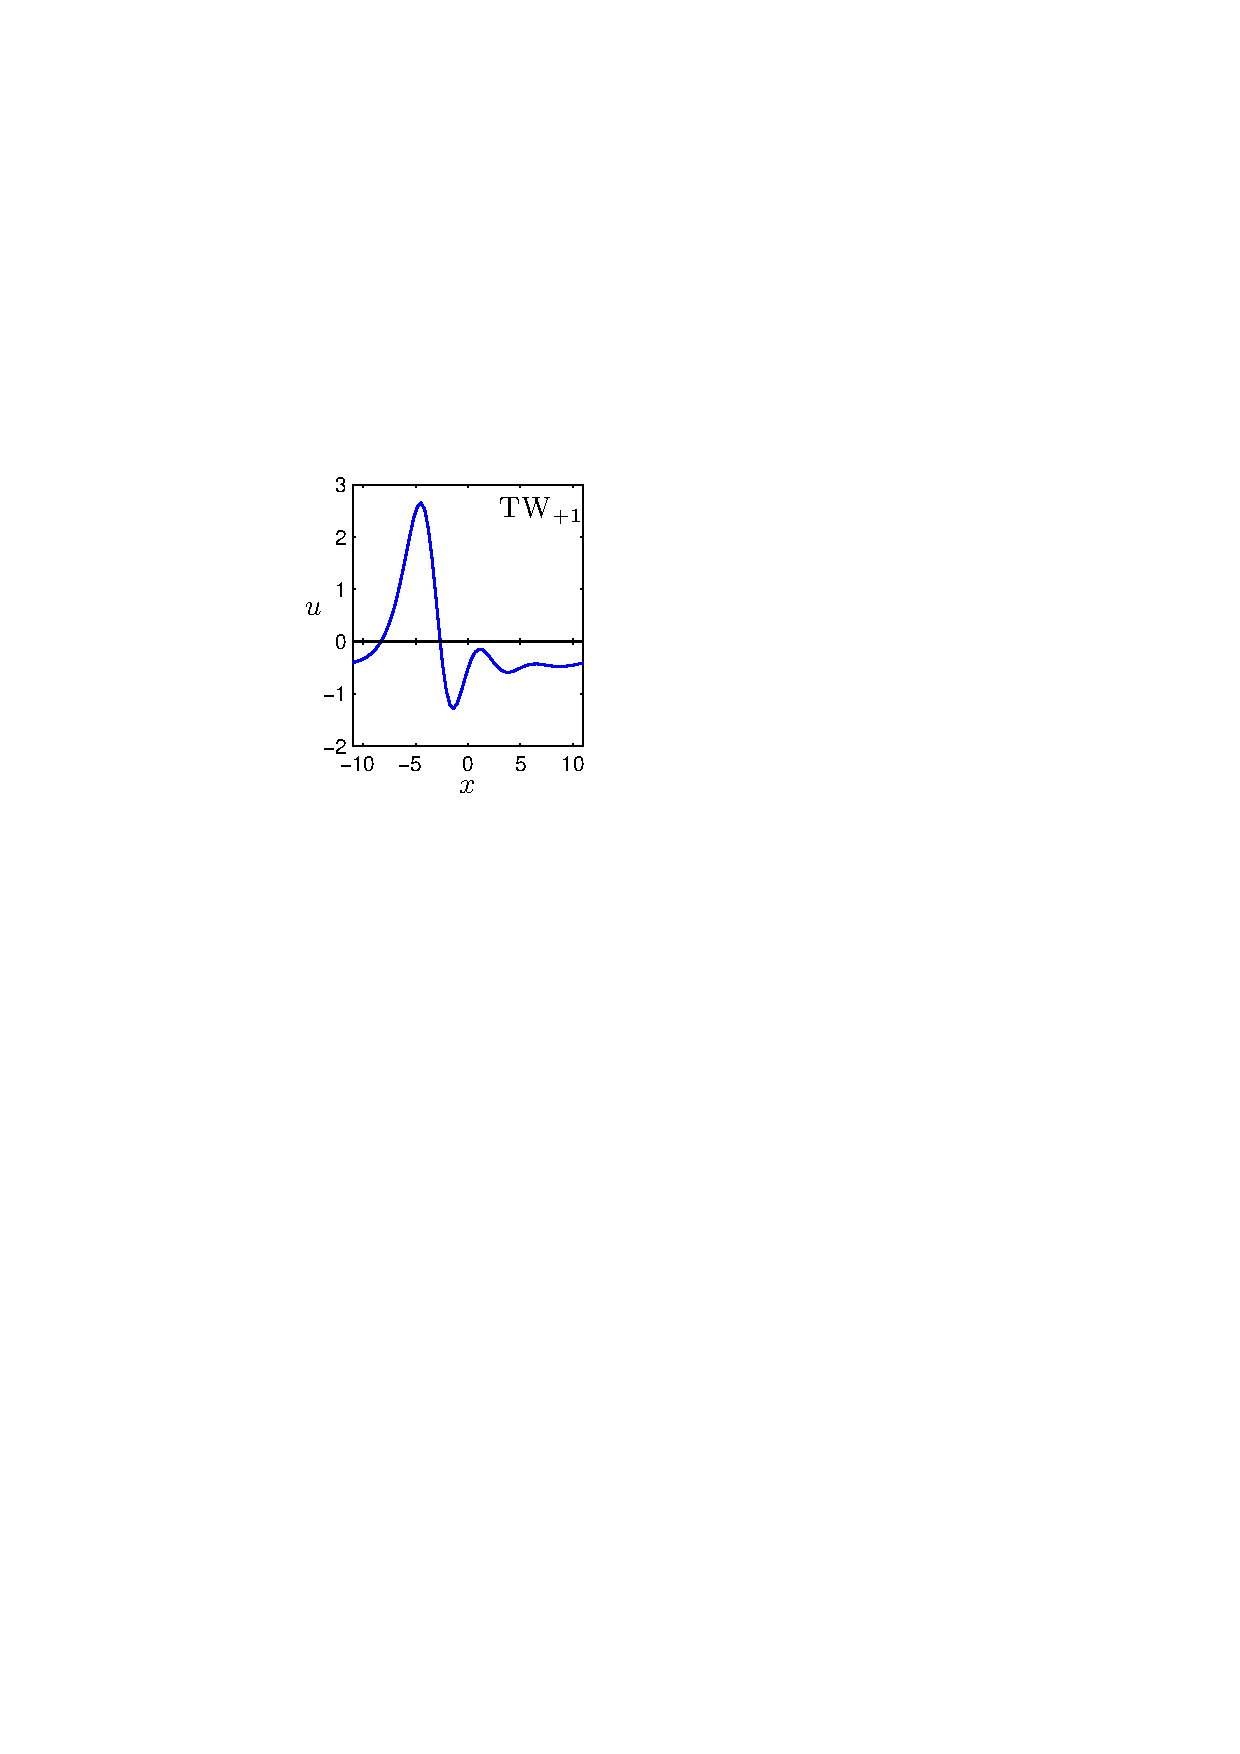
\includegraphics[width=0.6\textwidth,clip=true]{../../figs/ks22_TW1_profile}\\
 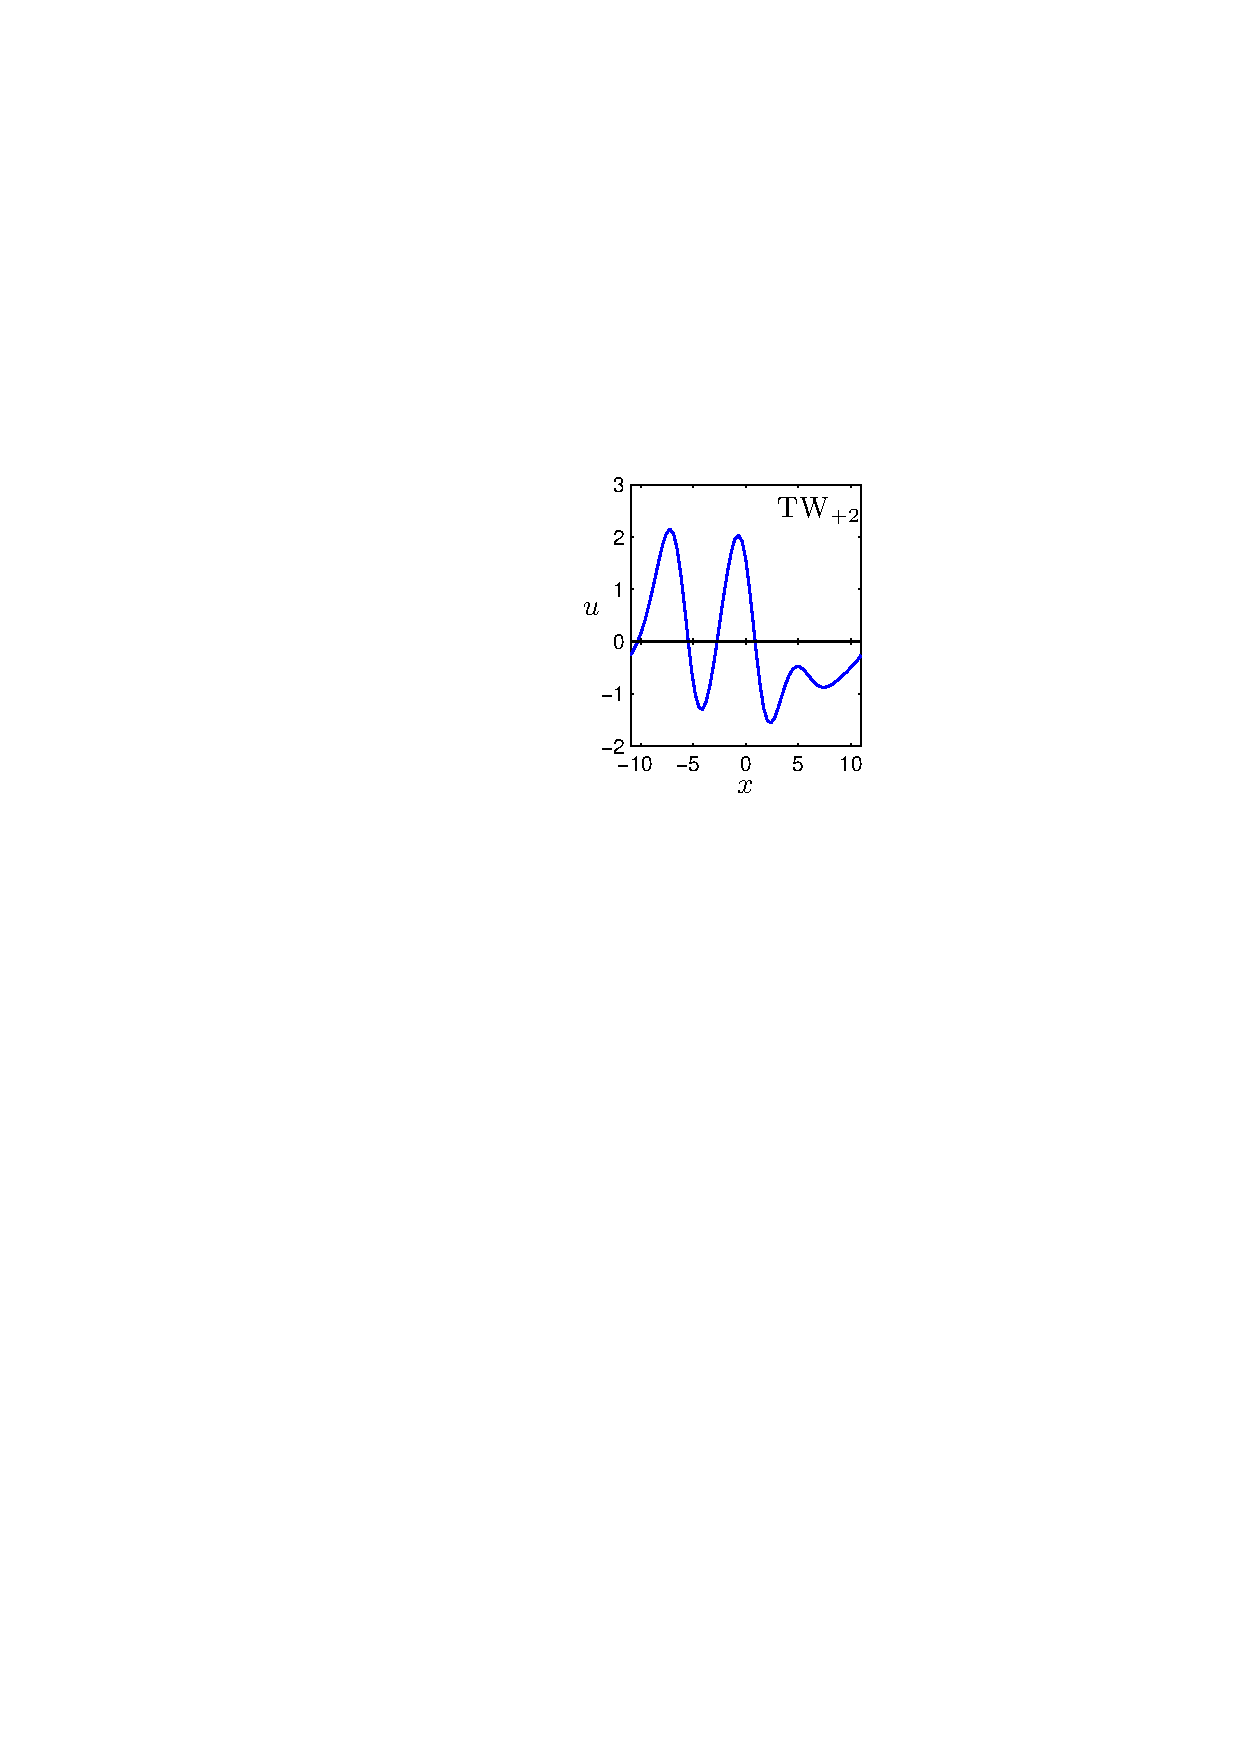
\includegraphics[width=0.6\textwidth,clip=true]{../../figs/ks22_TW2_profile}%\\
%  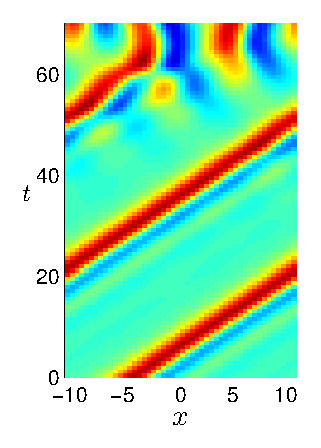
\includegraphics[width=0.5\textwidth,clip=true]{../../figs/ks22_TW1_orbit_c}
%  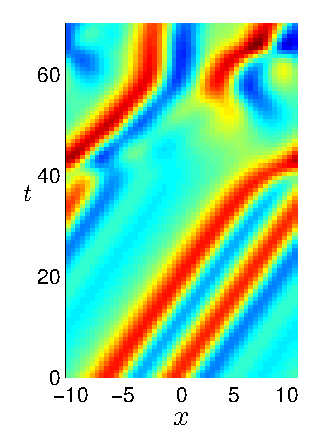
\includegraphics[width=0.5\textwidth,clip=true]{../../figs/ks22_TW2_orbit_c}
%  \end{tabular}
 \column{0.6\textwidth}
 \begin{itemize}
 \item Invariant (as a set) under rotations: relative equilibria.
 \item<alert@2-> They live in full space.

 \only<2->{
 \item
  Toshiba Corp and Microsoft Corp chairman Bill Gates are to
  work together to develop a next generation ``traveling-wave
  reactor'', which could operate for up to 100 years without
  refueling.
  \\{\footnotesize
    [news item - Tokyo, March 23, 2010]
    }
        }


\end{itemize}

 \end{columns}
\end{frame}


\begin{frame}{Unstable \rpo s}


\Rpo s (modulated traveling waves) satisfy:
\[
  \Shift_{\shift_p/L}u(x,\period{p}) =
  u(x+\shift_p,\period{p}) = u(x,0) = u_p(x)\,.
\]
\Po s satisfy:
% \[
%    \Refl u(x+\shift,\period{p}) =
%   -u(-x-\shift,\period{p}) = u(x+\shift,0) = u_p(x)
% \]
\[
   u(x,\period{p}) = u(x,0)=u_p(x)
\]

\end{frame}

\begin{frame}{A \rpo}
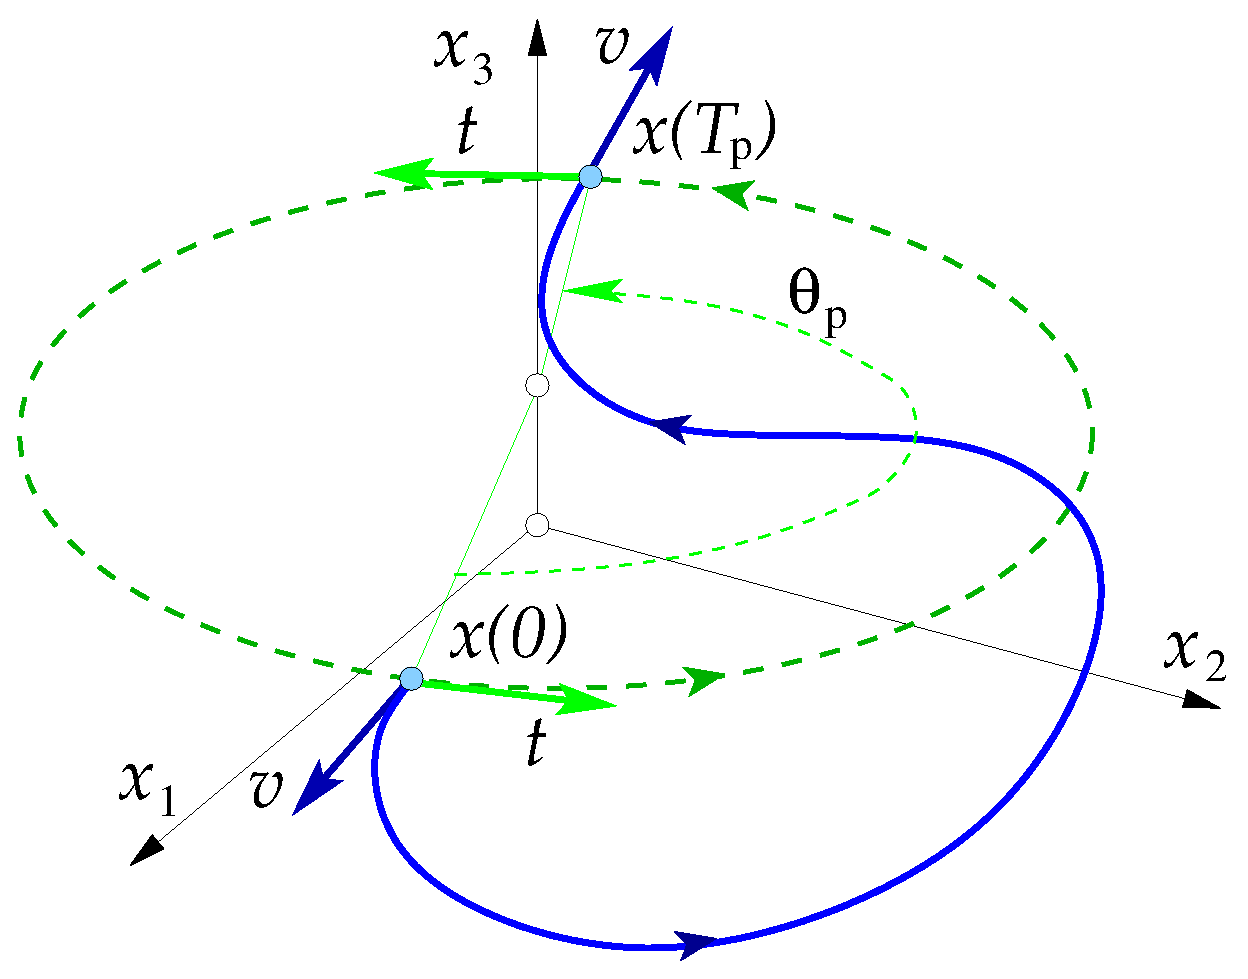
\includegraphics[width=0.8\textwidth,clip=true]{../../figs/rpo}
\end{frame}


\begin{frame}{Unstable \rpo s}

\scriptsize
 \begin{tabular}{ccccc}
~~~$\period{p} = 16.3$, & ~~~$\period{p} = 33.5$,  & ~~~$\period{p} = 47.6$,  &
%                          ~~~$\period{p} = 71.7$,  &
~~~$\period{p} = 10.3$ & ~~~$\period{p} = 33.4$\\
~~~$\shift_p = 2.86$ & ~~~$\shift_p = 4.04$ & ~~~$\shift_p = 5.68$ &
% ~~~$\shift_p = 5.503$ &
&\\
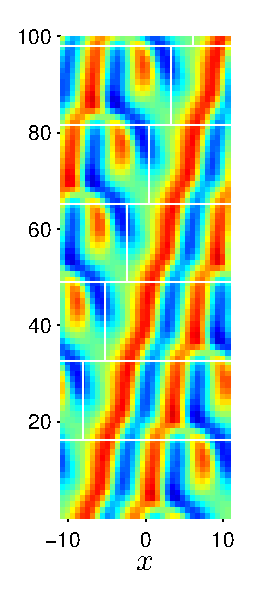
\includegraphics[width=0.15\textwidth,clip=true]{../../figs/ks22rpo016.3-02.86.eps}\hspace{-3ex} &
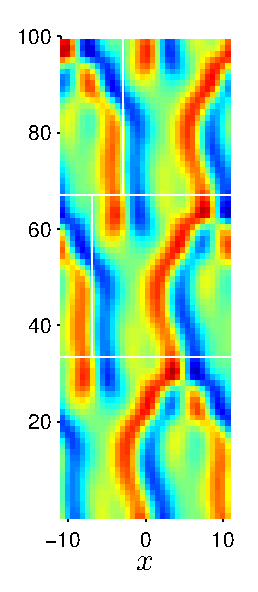
\includegraphics[width=0.15\textwidth,clip=true]{../../figs/ks22rpo033.5-04.04.eps}\hspace{-3ex} &
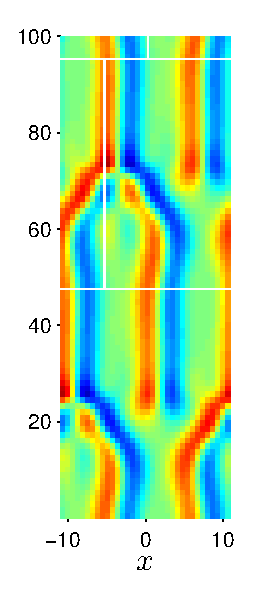
\includegraphics[width=0.15\textwidth,clip=true]{../../figs/ks22rpo047.6-05.68.eps}\hspace{-3ex} &
% 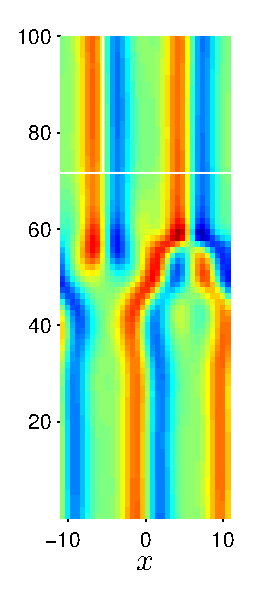
\includegraphics[width=0.15\textwidth,clip=true]{../../figs/ks22rpo071.7-05.50.eps}\hspace{-3ex} &
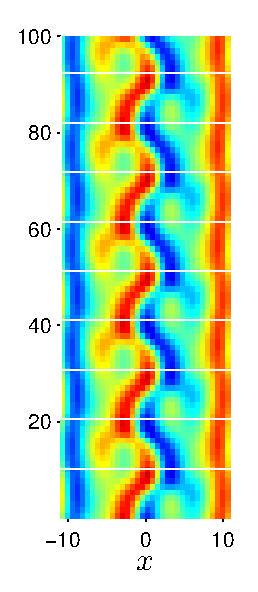
\includegraphics[width=0.15\textwidth,clip=true]{../../figs/ks22rpo020.5-00.00.eps}\hspace{-3ex} &
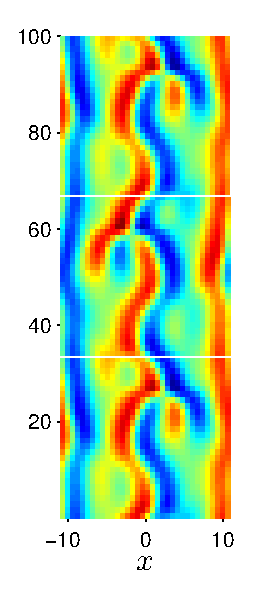
\includegraphics[width=0.15\textwidth,clip=true]{../../figs/ks22rpo066.8-00.00.eps}\\
% $\period{p} = 32.8$, $\shift_p = 10.96$ & $\period{p} = 34.6$, $\shift_p = 9.60$ & $\period{p} = 59.9$, $\shift_p = 5.44$ &
% $\period{p} = 84.4$, $\shift_p = 5.513$ & $\period{p} = 32.4$ & $\period{p} = 35.2$\\
% 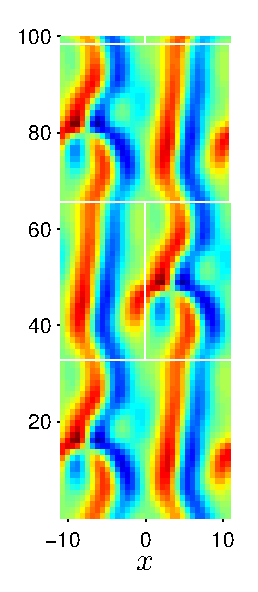
\includegraphics[width=0.15\textwidth,clip=true]{../../figs/ks22rpo032.8-10.96.eps}\hspace{-3ex} &
% 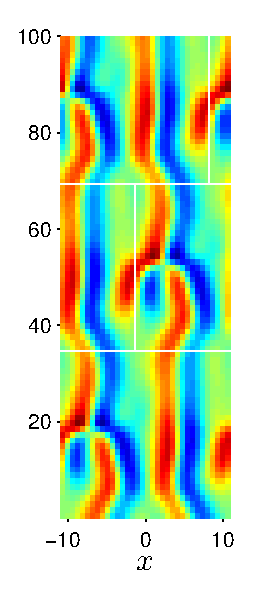
\includegraphics[width=0.15\textwidth,clip=true]{../../figs/ks22rpo034.6-09.60.eps}\hspace{-3ex} &
% 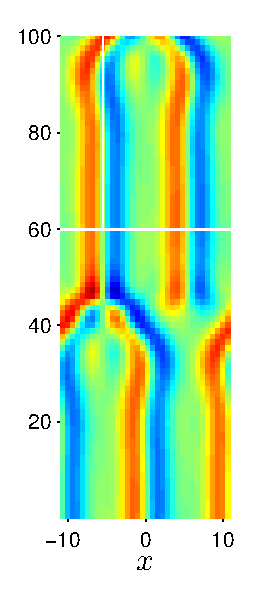
\includegraphics[width=0.15\textwidth,clip=true]{../../figs/ks22rpo059.9-05.44.eps}\hspace{-3ex} &
% 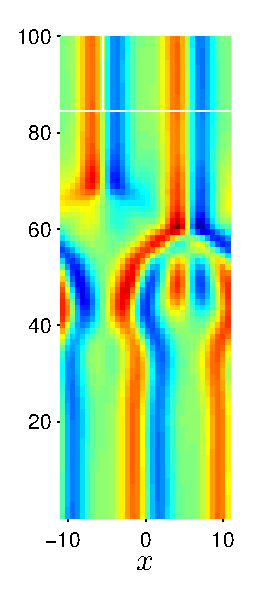
\includegraphics[width=0.15\textwidth,clip=true]{../../figs/ks22rpo084.4-05.51.eps}\hspace{-3ex} &
% 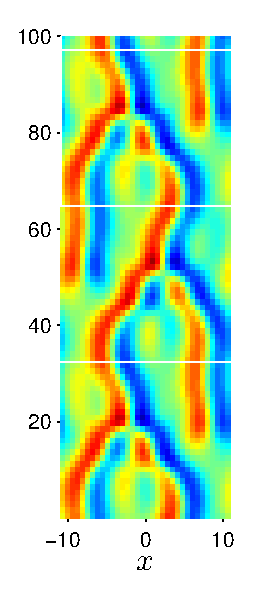
\includegraphics[width=0.15\textwidth,clip=true]{../../figs/ks22rpo064.7-00.00.eps}\hspace{-3ex} &
% 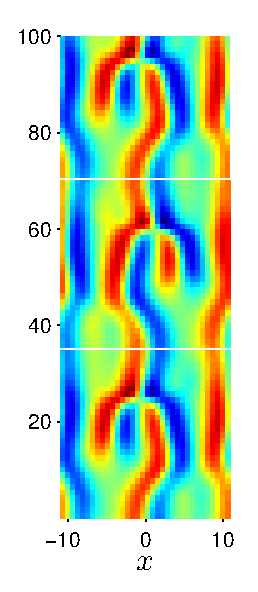
\includegraphics[width=0.15\textwidth,clip=true]{../../figs/ks22rpo070.3-00.00.eps}

\end{tabular}

\begin{itemize}
 \item Located 30,000 unstable periodic and \rpo s through multiple shooting.
 \item How are they organized?
\end{itemize}


\end{frame}

\begin{frame}{Linear stability of {\eqva} and \reqva.}
\begin{center} %\footnotesize
\begin{tabular}{cccc}
\EQV{1}& $\Re{\lambda}$ & $\Im{\lambda}$ & Symmetry \\\hline
   & $\ \ 0.1308$& $0.3341$ & -  \\
   & $\ \ 0.0824$& $0.3402$ & $\bbU$  \\
\EQV{2}&  &  & \\\hline
   & $\ \ 0.1390$& $0.2384$ & $\bbU$         \\
\EQV{3}&  &   \\\hline
     &$\ \ 0.0933$&          & $\bbU$     \\
     &$\ \ 0.0933$&          & -           \\
$\REQV{\pm}{1}$&  &   \\\hline
   & $\ \ 0.1156$ & $0.8173$ & -  \\
   & $\ \ 0.0337$ & $0.4189$ & -  \\
$\REQV{\pm}{2}$&  &   \\\hline
     & $\ \ 0.3370$ &          & -  \\
\end{tabular}
\end{center}
%   \column{0.5\textwidth}
%   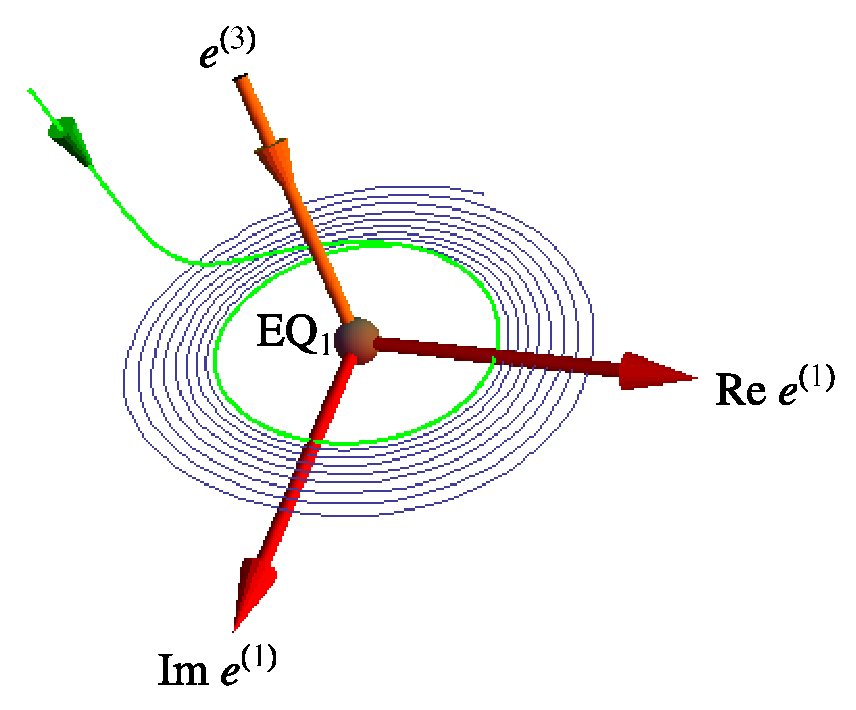
\includegraphics[width=\textwidth, clip=true]{../../figs/lorenzPolarManifDetail1.eps}
\end{frame}

\section{Symmetry reduction}

\subsection{Reduction methods}

\begin{frame}{Symmetry reduction}
\begin{itemize}
 \item All points related by a symmetry operation are mapped to the same point.
 \item Relative equilibria become equilibria and relative periodic orbits become periodic orbits in reduced space.
 \item Families of solutions are mapped to a single solution.
\end{itemize}
\end{frame}


\begin{frame}{Reduction methods}

\begin{itemize}
	\item Integrate in directions transverse to the direction
of group action at a point $x_0$. \textcolor{red}{Local.}\\
	(Rowley and Marsden (2000)).
\end{itemize}

\end{frame}

\begin{frame}{Reduction methods}

\begin{itemize}
 \item<alert@2-> rewrite the equations in variables invariant
 under the symmetry transformation
 \only<2->{\item or compute solutions in original space and map them to invariant variables.}
 \only<3->{\item how do we find those variables?
	\begin{itemize}
	\item<alert@4-> Invariant polynomials (Hilbert basis)\only<3>{.}\only<4->{: computationaly prohibitive for high-dimensional flows.}
	\only<5->{\item<alert@6-> Moving frame method by Cartan, reformulated by Fels and Olver (1999)\only<5>{.}}\only<6->{: singularities.}
	\end{itemize}
 }
\end{itemize}

\end{frame}

% \begin{frame}{Moving frame method}
%  \begin{block}{Idea}
%   	\begin{itemize}
%  		\item Introduce a \emph{cross-section}: A hypersurface that intersects all group
% 			orbits of a point exactly once.
% 		\item Then given a point $x$ find a map that tells you the transformation parameter(s)
% 			needed to bring $x$ to the cross-section. This is called a moving frame.
% 	\end{itemize}
%  \end{block}
%
%  \begin{block}{For \CLe}
% 	\begin{description}
%  		\item{Cross-section} $x_1=0$, $x_2>0$.
% 		\item{Moving frame} $\theta=\tan^{-1}\frac{x_1}{x_2}$.
% 	\end{description}
%   	
%  \end{block}


% \end{frame}

% \begin{frame}{Moving frame method}
%
% % \[
% % 	\left(\barr{cc} \overline{b}_k \\ \overline{c}_k\earr \right)=\left(\barr{cc}
% % 			    			\cos(k\theta) & -\sin(k\theta)\\
% % 						\sin(k\theta) & \cos(k\theta)\\
% % 			   			\earr\\	
% % 						\right) \left(\barr{cc} b_k \\ c_k\earr\right)\,,\ \ k=1,\ldots N\,.
% % \]
% % with $a_k=b_k+i c_k\,,\ b_k,c_k\in\Rls{}$.
% \end{frame}

\begin{frame}{Moving frame method}
  \begin{block}{}
	\begin{itemize}
	\item Write out group transformations explicitly:
	\[
	 \left(\barr{cc} \overline{b}_k \\ \overline{c}_k\earr \right)=\left(\barr{cc}
			    			\cos(k\theta) & -\sin(k\theta)\\
						\sin(k\theta) & \cos(k\theta)\\
			   			\earr	
						\right)\left(\barr{cc} b_k \\ c_k\earr\right)\,,\ \ k=1,\ldots N\,.
	\]
	\item Define a \emph{cross-section}:
	\[
 		K_1(a)=c_1=0\,,\qquad b_1>0\,
	\]
	\item Find the group element that brings a point back to the cross-section:
	\[
		\theta=-\tan^{-1}\frac{c_1}{b_1}\,,	
	\]
	\end{itemize}
  \end{block}
\end{frame}

\begin{frame}{Invariants}
  \begin{block}{}
\only<1>{
	\[
	\begin{array}{ll}
	u_1=r_1=\sqrt{b_1^2+c_1^2}&  \\
	u_3=\frac{b_2 \left(b_1^2-c_1^2\right)+2 b_1 c_1 c_2}{r_1^2}& \\
	u_4=\frac{-2
	b_1 b_2 c_1+\left(b_1^2-c_1^2\right) c_2}{r_1^2} & \\
	u_5=\frac{b_1 b_3 \left(b_1^2-3 c_1^2\right)-c_1 \left(-3
	b_1^2+c_1^2\right) c_3}{r_1^3}& \\

	u_6=\frac{-3 b_1^2 b_3 c_1+b_3 c_1^3+b_1^3 c_3-3 b_1 c_1^2 c_3}{r_1^3} & \\
	u_7=\frac{b_4
 	\left(b_1^4-6 b_1^2 c_1^2+c_1^4\right)+4 b_1 c_1 \left(b_1^2-c_1^2\right) c_4}{r_1^4}& \\
	u_8=\frac{4 b_1
 	b_4 c_1 \left(-b_1^2+c_1^2\right)+\left(b_1^4-6 b_1^2 c_1^2+c_1^4\right) c_4}{r_1^4}
% \\ u_9=\frac{b_1
% 	b_5 \left(b_1^4-10 b_1^2 c_1^2+5 c_1^4\right)+c_1 \left(5 b_1^4-10 b_1^2 c_1^2+c_1^4\right) c_5}{r_1^5}&u_{10}=\frac{-b_5
% 	c_1 \left(5 b_1^4-10 b_1^2 c_1^2+c_1^4\right)+b_1 \left(b_1^4-10 b_1^2 c_1^2+5 c_1^4\right) c_5}{r_1^5}\\ u_{11}=\frac{b_6
% 	\left(b_1^6-15 b_1^4 c_1^2+15 b_1^2 c_1^4-c_1^6\right)+2 b_1 c_1 \left(3 b_1^4-10 b_1^2 c_1^2+3 c_1^4\right) c_6}{r_1^6}&u_{12}=\frac{-2
% 	b_1 b_6 c_1 \left(3 b_1^4-10 b_1^2 c_1^2+3 c_1^4\right)+\left(b_1^6-15 b_1^4 c_1^2+15 b_1^2 c_1^4-c_1^6\right) c_6}{r_1^6}\\
	\end{array}
	\]
}
  \end{block}

\end{frame}

\section[Conclusions]{Conclusions-Future work}

 \begin{frame}{Conclusions and future work}

\begin{block}{Conclusion}
  \begin{itemize}
   \item Symmetry reduction: efficient implementation allows
   exploration of high-dimensional flows with continuous
   symmetry.
   \item We develop an understanding of how the stretching and folding
  	of unstable manifolds in \KSe\ organizes the flow.
  \end{itemize}
\end{block}


\begin{block}{Future work}
\begin{itemize}
  \item Construct Poincar\'e sections and return maps.
  \item Find all (relative) periodic orbits up to a given period.
  \item Use the information quantitatively (periodic orbit theory).
\end{itemize}
\end{block}

\end{frame}

\end{document}
